\section{Architectural Design}

Basic framework to identify music in radio broadcasts is proposed in 
\say{Radio Broadcast Monitoring to Ensure Copyright Ownership}\cite{Nishan}. And it's currently
implemented and deployed in \ac{osca}. Hence the infrastructure to contain the basic framework
of a radio monitoring system is already there. When different methods of music identification
are applied to radio broadcast monitoring, only registering service, database and matching service
will be changed conserving the other modules that are in the architecture as shown in the Figure
\ref{fig:new_arch}.

\begin{figure}[H]
    \centering
    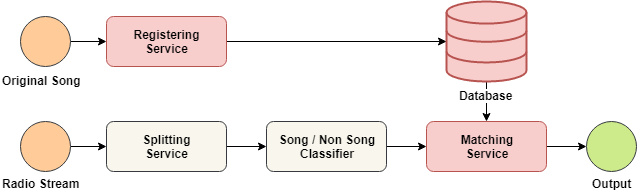
\includegraphics[scale=0.6]{NewSystem.png}
    \caption{Architectural Design}
    \label{fig:new_arch}
\end{figure}

Registering service takes original songs as input and generate specific descriptors to be stored
in the database. Database stores the generated audio descriptors by registering service in
retrieval friendly framework to help matching service to retrieve descriptors faster. Matching
service takes a query audio clip and determine whether that query audio clip contains song registered
before.     